\documentclass[polish,a4paper,11pt]{mwart}

\usepackage[polish]{babel}
\usepackage[utf8]{inputenc}
\usepackage{polski}
\usepackage[T1]{fontenc}
\usepackage{lmodern}  % zestaw fontów
\usepackage{indentfirst}
\frenchspacing

\usepackage{enumerate}
\usepackage{graphicx}
\usepackage{float}
\usepackage{makecell}
\usepackage{siunitx}
\sisetup{output-decimal-marker = {,}}
\usepackage{icomma}
\let\lll\undefined
\usepackage{amsmath, amssymb, amsfonts}
\usepackage{mathtools}
\usepackage{import}		% wklejanie pdf_tex
\usepackage{xcolor}		% kolory
\usepackage{multirow}
\usepackage{microtype}
\usepackage{tabularx}

\usepackage{csquotes}
\DeclareQuoteAlias{croatian}{polish}

\usepackage{placeins}	% poprawia float

\let\Oldsection\section
\renewcommand{\section}{\FloatBarrier\Oldsection}

\let\Oldsubsection\subsection
\renewcommand{\subsection}{\FloatBarrier\Oldsubsection}

\let\Oldsubsubsection\subsubsection
\renewcommand{\subsubsection}{\FloatBarrier\Oldsubsubsection}

\AtBeginDocument{
  \renewcommand{\tablename}{Tab.}
  \renewcommand{\figurename}{Rys.}
}

\setlength{\emergencystretch}{3em}

\DeclareSIUnit\decibelV{dBV}

\date{\today}
\author{Zuzanna Kusal, Szymon Mikulicz, Marcel Piszak, Anna Warowny}
\title{Sprawozdanie z projektu redukcji drgań płyty}

\begin{document}

\maketitle

\section{Cel}

Celem projektu była redukcja drgań płyty kwadratowej, jednostronnie
utwierdzonej, pobudzonej do drgań w częstotliwościach własnych.

\section{Przebieg}

\begin{figure}[!tbh]
  \centering
  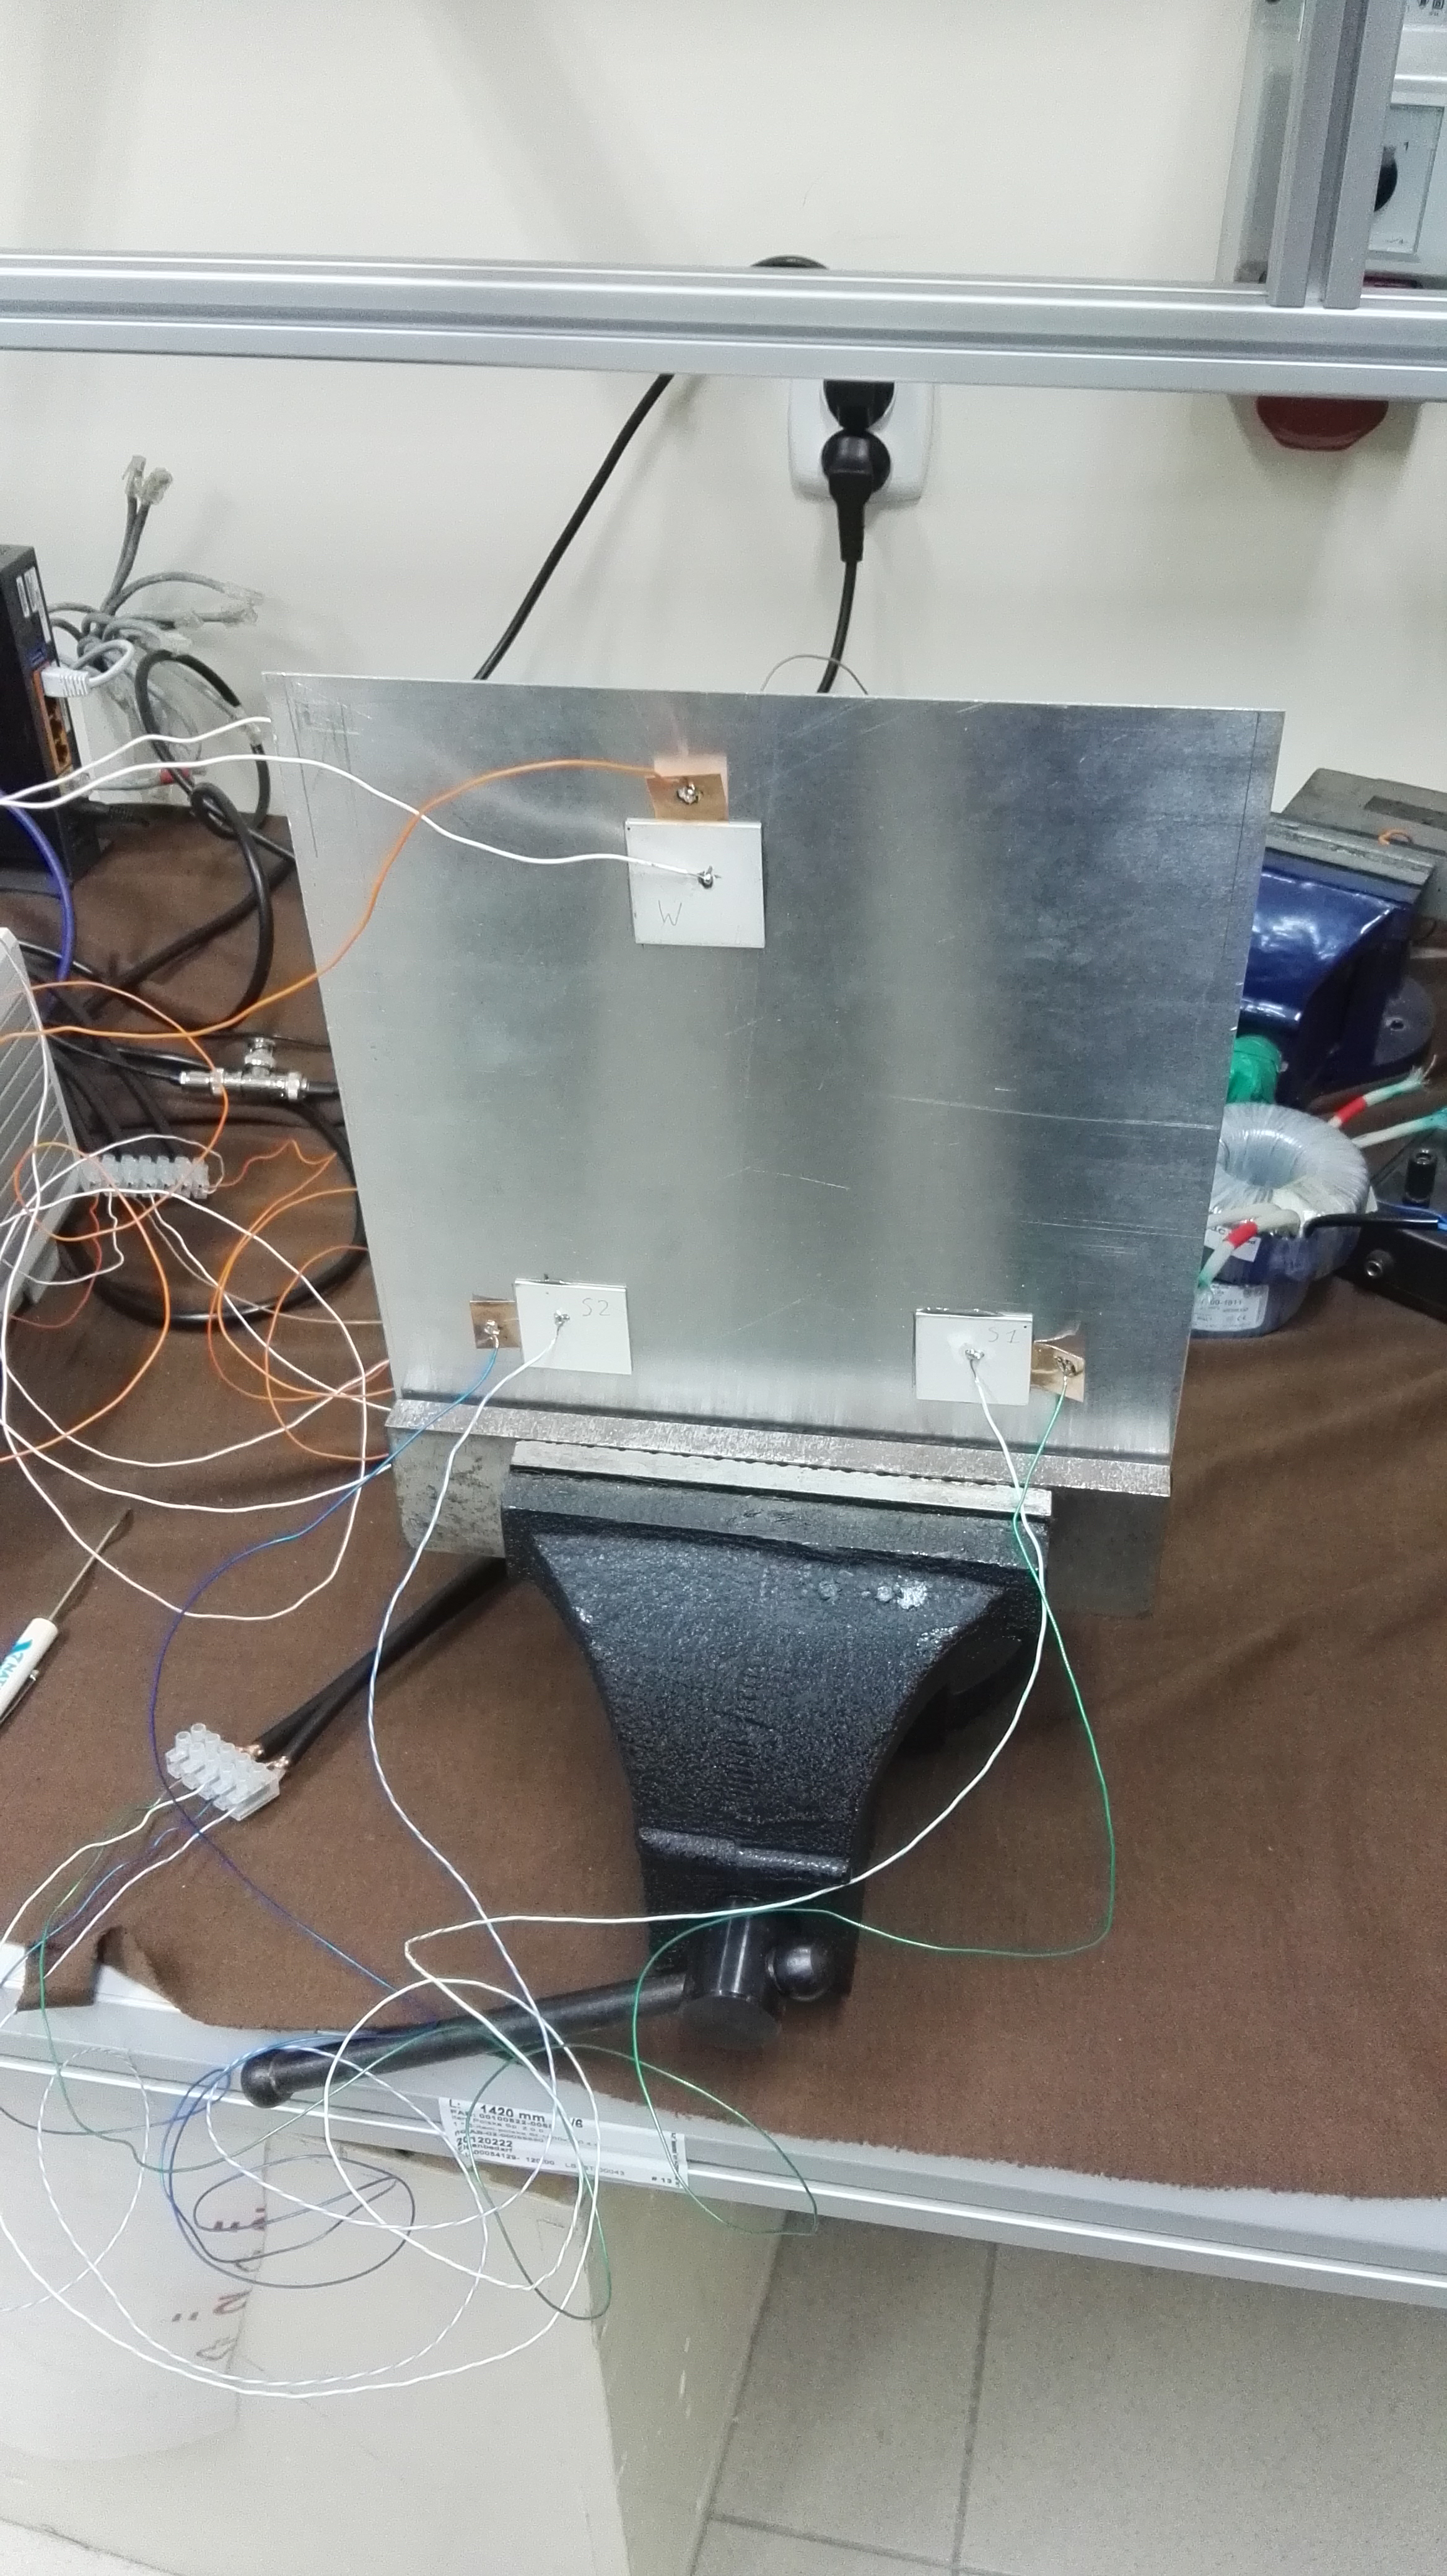
\includegraphics[width=\textwidth]{./bitgraphics/plate1.jpg}
  \caption{Widok na wzbudnik oraz czujniki zainstalowane na płycie}
  \label{fig:plate1}
\end{figure}

\begin{figure}[!tbh]
  \centering
  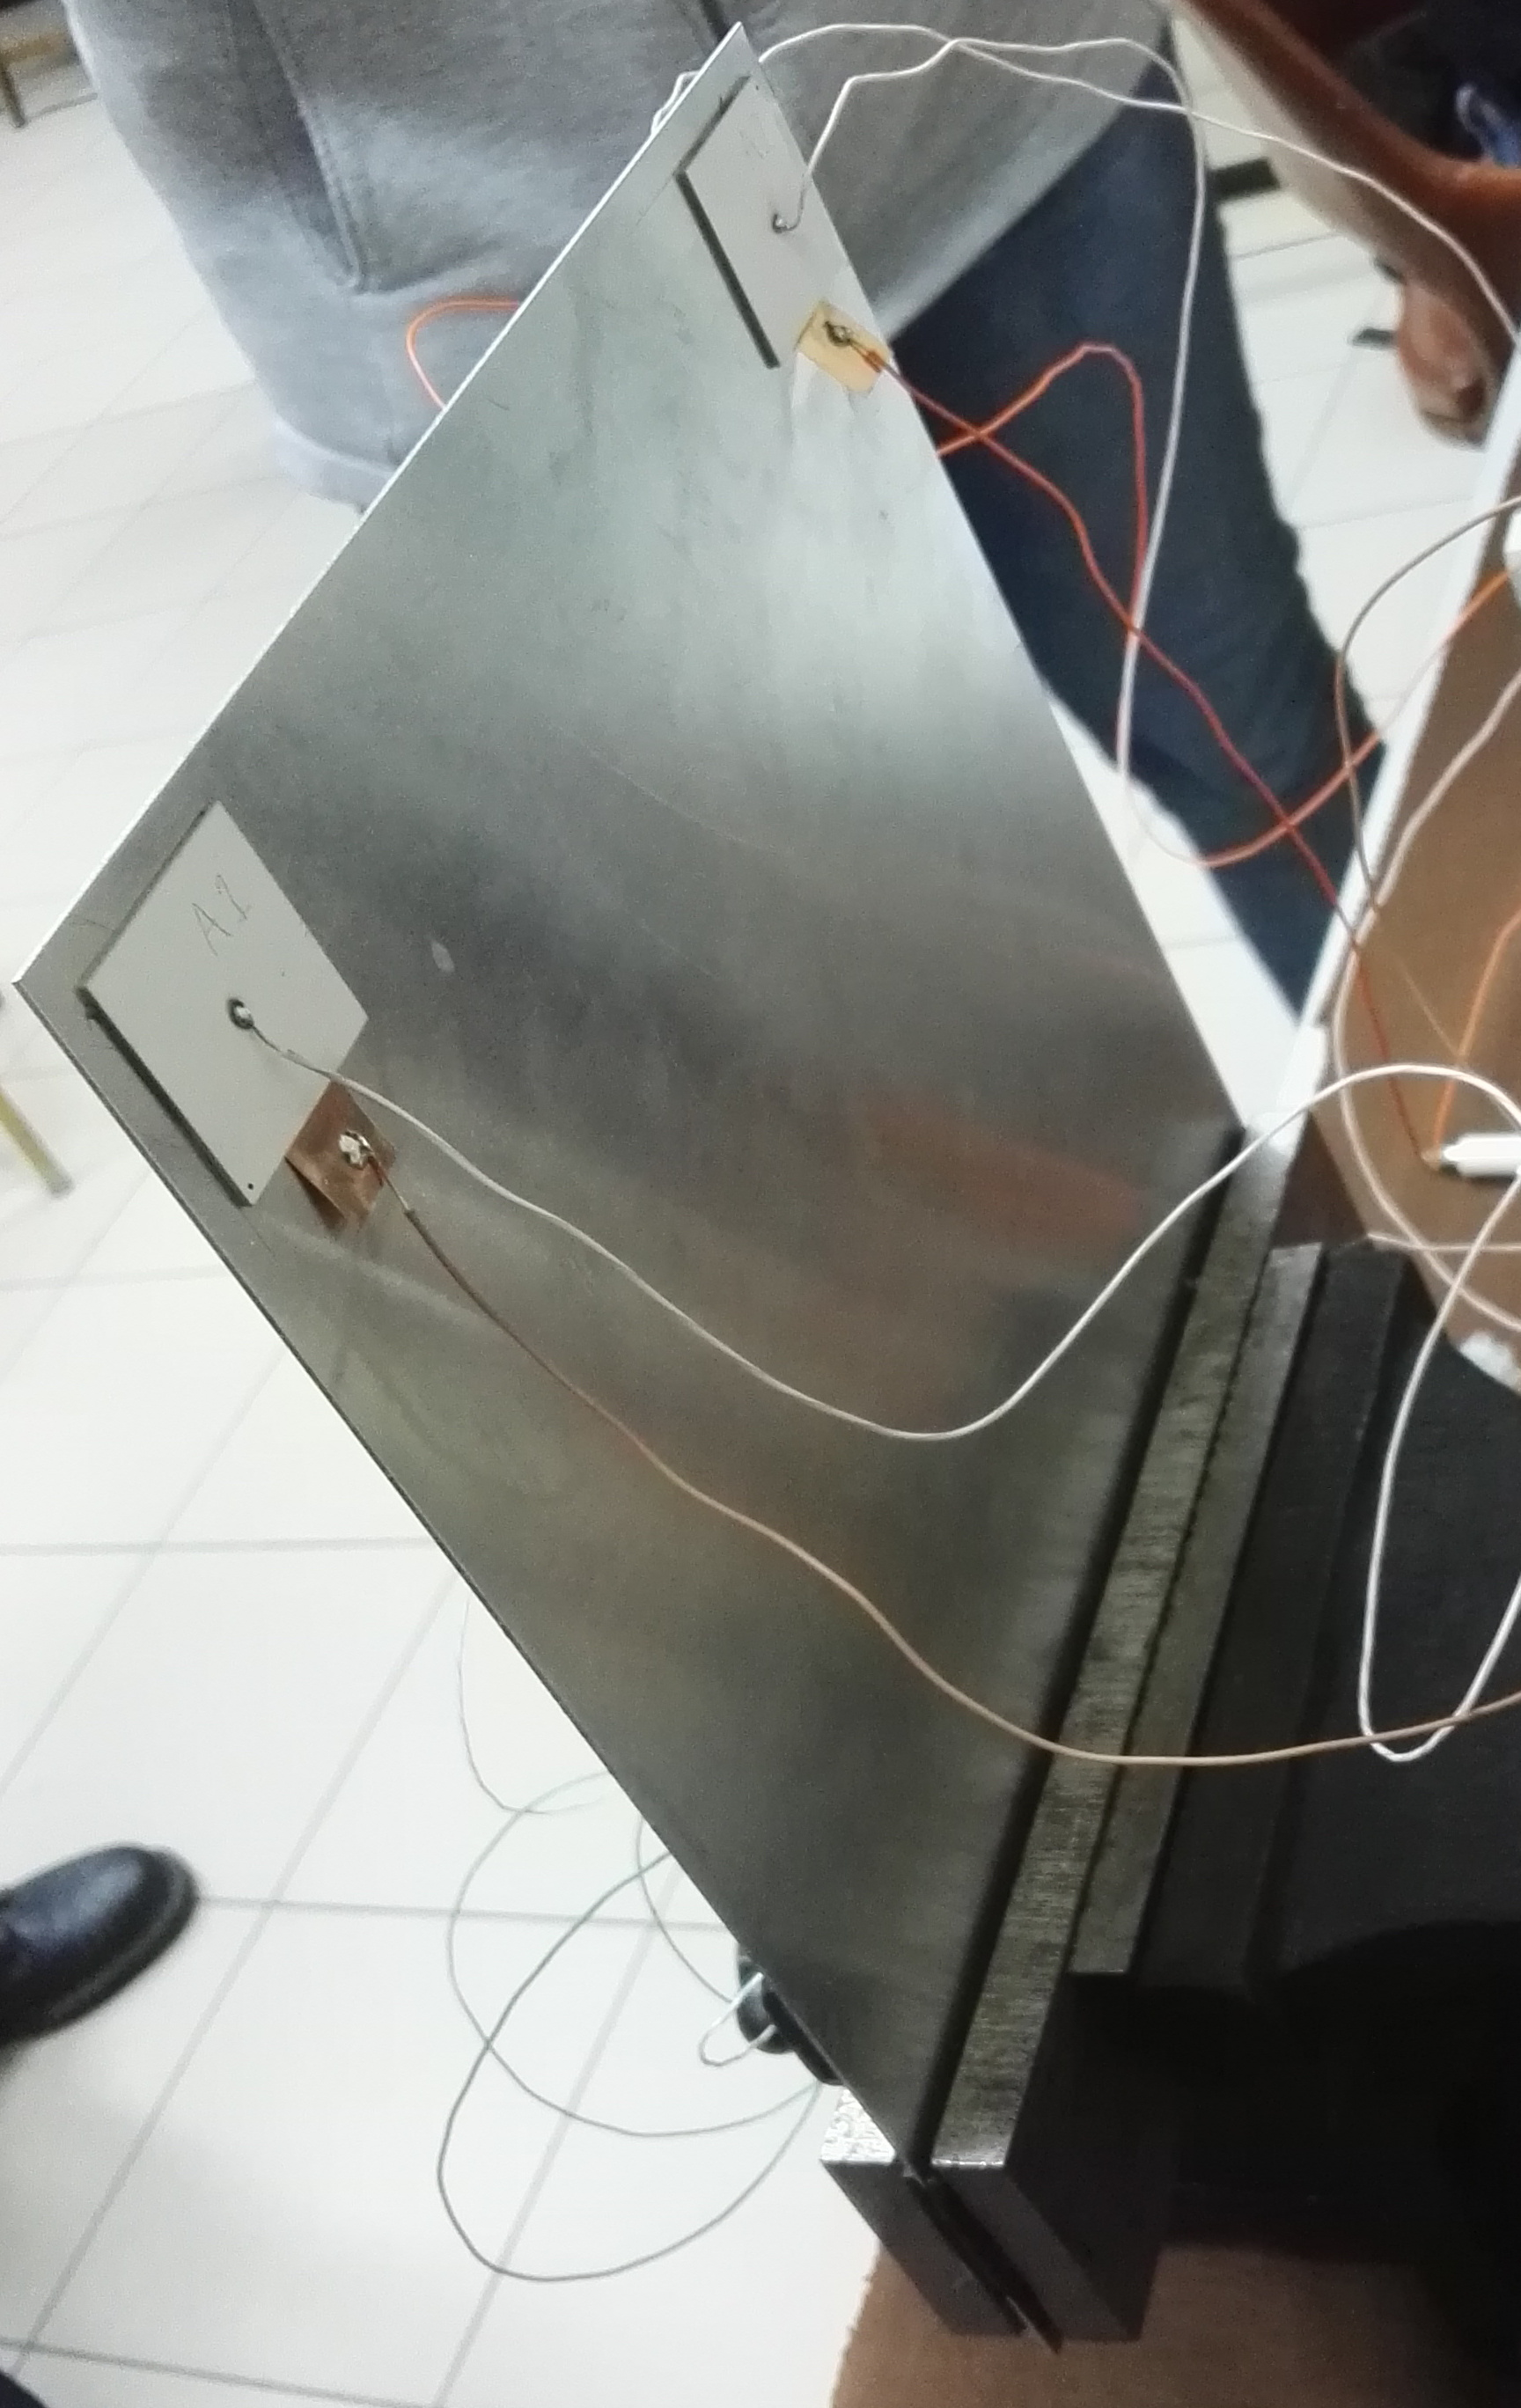
\includegraphics[width=0.7\textwidth]{./bitgraphics/plate2.jpg}
  \caption{Widok na aktuatory zainstalowane na płycie}
  \label{fig:plate2}
\end{figure}

\section{Identyfikacja częstotliwości własnych}


\section{Wyniki}

\begin{table}[!tbh]
  \centering
  \caption{Częstotliwości wybranych modów drgań płyty}
  \begin{tabular}{|c|c|c|c|c|c|}
    \hline
    Numer modu & () & () & () & () & () \\
    \hline
    $f_{wlas} [\si{\hertz}]$ & 250 & 300 & 570 & 710 & 920\\
    \hline
  \end{tabular}
  \label{tab:czest}
\end{table}

\begin{table}[!tbh]
  \centering
  \caption{Wyniki redukcji drgań dla modu \SI{250}{\hertz}}
  \label{tab:red1}
  \begin{tabular}{|c|c|c|c|c|c|c|}
    \cline{3-7}
    \multicolumn{2}{c|}{}&\multicolumn{2}{c|}{Aktuator}&\multicolumn{3}{c|}{Czujnik [\si{\decibelV}]}\\\cline{3-7}
    \multicolumn{2}{c|}{}&$A1$&$A2$&$S1$&$S2$&$S1+S2$\\\hline
    \multirow{2}{*}{tło}               &   $A [\si{\V}]$ & - & - & -84,0 & -90,2 & -83,3 \\\cline{2-7}
				       &$\Phi [\si{\degree}]$ & - & - & \multicolumn{3}{c}{}\\\hline
    \multirow{2}{*}{bez redukcji}      &   $A [\si{\V}]$ & - & - & -19,0 & -34,5 & -18,8 \\\cline{2-7}
				       &$\Phi [\si{\degree}]$ & - & - & \multicolumn{3}{c}{}\\\hline
    \multirow{6}{*}{$\min\{S1\}$}      &   $A [\si{\V}]$ & 2,92 & - & \textbf{-63,5} & -52,1 & -51,8 \\\cline{2-7}
				       &$\Phi [\si{\degree}]$ & 15 & - & \multicolumn{3}{c}{}\\\cline{2-7}
				       &   $A [\si{\V}]$ & - & 3,42 & \textbf{-59,2} & -42,9 & -42,8 \\\cline{2-7}
				       &$\Phi [\si{\degree}]$ & - & 24 & \multicolumn{3}{c}{}\\\cline{2-7}
				       &   $A [\si{\V}]$ & 2,8 & 0,2 & \textbf{-55,0} & -51,1 & -49,6 \\\cline{2-7}
				       &$\Phi [\si{\degree}]$ & 18 & 333 & \multicolumn{3}{c}{}\\\hline
    \multirow{6}{*}{$\min\{S2\}$}      &   $A [\si{\V}]$ & 2,78 & - & -36,0 & \textbf{-73,3} & -36,0\\\cline{2-7}
				       &$\Phi [\si{\degree}]$ & 10 & - & \multicolumn{3}{c}{}\\\cline{2-7}
				       &   $A [\si{\V}]$ & - & 3,1 & -26,8 & \textbf{-67,3} & -26,8 \\\cline{2-7}
				       &$\Phi [\si{\degree}]$ & - & 0 & \multicolumn{3}{c}{}\\\cline{2-7}
				       &   $A [\si{\V}]$ & 2,55 & 0,29 & -36,4 & \textbf{-80,1} & -36,4 \\\cline{2-7}
				       &$\Phi [\si{\degree}]$ & 6 & 69 & \multicolumn{3}{c}{}\\\hline
    \multirow{6}{*}{$\min\{S1+S2\}$}   &   $A [\si{\V}]$ & 2,92 & - & -63,5  & -52,1 & \textbf{-51,8}\\\cline{2-7}
				       &$\Phi [\si{\degree}]$ & 15 & - & \multicolumn{3}{c}{}\\\cline{2-7}
				       &   $A [\si{\V}]$ & - & 3,46 & -62,8 & -42,0 & \textbf{-42,0} \\\cline{2-7}
				       &$\Phi [\si{\degree}]$ & - & 23 & \multicolumn{3}{c}{}\\\cline{2-7}
				       &   $A [\si{\V}]$ & 2,92 & 0 & -63,5 & -52,1 & \textbf{-51,8} \\\cline{2-7}
				       &$\Phi [\si{\degree}]$ & 15 & 0 & \multicolumn{3}{c}{}\\\cline{1-4}
  \end{tabular}
\end{table}

\begin{table}[!tbh]
  \centering
  \caption{Wyniki redukcji drgań dla modu \SI{300}{\hertz}}
  \label{tab:red2}
  \begin{tabular}{|c|c|c|c|c|c|c|}
    \cline{3-7}
    \multicolumn{2}{c|}{}&\multicolumn{2}{c|}{Aktuator}&\multicolumn{3}{c|}{Czujnik [\si{\decibelV}]}\\\cline{3-7}
    \multicolumn{2}{c|}{}&$A1$&$A2$&$S1$&$S2$&$S1+S2$\\\hline
    \multirow{2}{*}{tło}               &   $A [\si{\V}]$ & - & - & -100,0 & -99,0 & -99,0 \\\cline{2-7}
				       &$\Phi [\si{\degree}]$ & - & - & \multicolumn{3}{c}{}\\\hline
    \multirow{2}{*}{bez redukcji}      &   $A [\si{\V}]$ & - & - & -19,9 & -40,0 & -19,9 \\\cline{2-7}
				       &$\Phi [\si{\degree}]$ & - & - & \multicolumn{3}{c}{}\\\hline
    \multirow{6}{*}{$\min\{S1\}$}      &   $A [\si{\V}]$ & 4,5 & - & \textbf{-21,2} & -43,7 & -21,2\\\cline{2-7}
				       &$\Phi [\si{\degree}]$ & 286 & - & \multicolumn{3}{c}{}\\\cline{2-7}
				       &   $A [\si{\V}]$ & - & \textcolor{red}{4} & \textbf{-22,0} & -43,5 & -22,0 \\\cline{2-7}
				       &$\Phi [\si{\degree}]$ & - & 180 & \multicolumn{3}{c}{}\\\cline{2-7}
				       &   $A [\si{\V}]$ & 5 & \textcolor{red}{4} & \textbf{-24,2} & -52,0 & -24,2 \\\cline{2-7}
				       &$\Phi [\si{\degree}]$ & 290 & 180 & \multicolumn{3}{c}{}\\\hline
    \multirow{6}{*}{$\min\{S2\}$}      &   $A [\si{\V}]$ & \textcolor{red}{5,1} & - & -21,5 & \textbf{-44,7} & -21,5 \\\cline{2-7}
				       &$\Phi [\si{\degree}]$ & 291 & - & \multicolumn{3}{c}{}\\\cline{2-7}
				       &   $A [\si{\V}]$ & - & \textcolor{red}{4} & -21,5 & \textbf{-44,6} & -21,4 \\\cline{2-7}
				       &$\Phi [\si{\degree}]$ & - & 210 & \multicolumn{3}{c}{}\\\cline{2-7}
				       &   $A [\si{\V}]$ & \textcolor{red}{5,1} & \textcolor{red}{4} & -23,7 & \textbf{-59,5} & -13,7\\\cline{2-7}
				       &$\Phi [\si{\degree}]$ & 291 & 211 & \multicolumn{3}{c}{}\\\hline
    \multirow{6}{*}{$\min\{S1+S2\}$}   &   $A [\si{\V}]$ & \textcolor{red}{5,1} & - & -29,7 & -45,0 & \textbf{-21,7}\\\cline{2-7}
				       &$\Phi [\si{\degree}]$ & 292 & - & \multicolumn{3}{c}{}\\\cline{2-7}
				       &   $A [\si{\V}]$ & - & \textcolor{red}{4} & -22,0 & -43,6 & \textbf{-22,0} \\\cline{2-7}
				       &$\Phi [\si{\degree}]$ & - & 180 & \multicolumn{3}{c}{}\\\cline{2-7}
				       &   $A [\si{\V}]$ & \textcolor{red}{5,1} & \textcolor{red}{4} & -24,5 & -51,3 & \textbf{-24,5} \\\cline{2-7}
				       &$\Phi [\si{\degree}]$ & 294 & 180 & \multicolumn{3}{c}{}\\\cline{1-4}
  \end{tabular}
\end{table}

\begin{table}[!tbh]
  \centering
  \caption{Wyniki redukcji drgań dla modu \SI{570}{\hertz}}
  \label{tab:red3}
  \begin{tabular}{|c|c|c|c|c|c|c|}
    \cline{3-7}
    \multicolumn{2}{c|}{}&\multicolumn{2}{c|}{Aktuator}&\multicolumn{3}{c|}{Czujnik [\si{\decibelV}]}\\\cline{3-7}
    \multicolumn{2}{c|}{}&$A1$&$A2$&$S1$&$S2$&$S1+S2$\\\hline
    \multirow{2}{*}{tło}               &   $A [\si{\V}]$ & - & - & -82,7 & -97,5 & -82,8 \\\cline{2-7}
				       &$\Phi [\si{\degree}]$ & - & - & \multicolumn{3}{c}{}\\\hline
    \multirow{2}{*}{bez redukcji}      &   $A [\si{\V}]$ & - & - & -10,2 & -31,5 & -10,2 \\\cline{2-7}
				       &$\Phi [\si{\degree}]$ & - & - & \multicolumn{3}{c}{}\\\hline
    \multirow{6}{*}{$\min\{S1\}$}      &   $A [\si{\V}]$ & 4,4 & - & \textbf{-54,5} & -38,0 & -37,9 \\\cline{2-7}
				       &$\Phi [\si{\degree}]$ & 26 & - & \multicolumn{3}{c}{}\\\cline{2-7}
				       &   $A [\si{\V}]$ & - & 3,57 & \textbf{-40,5} & -33,9 & -33 \\\cline{2-7}
				       &$\Phi [\si{\degree}]$ & - & 355 & \multicolumn{3}{c}{}\\\cline{2-7}
				       &   $A [\si{\V}]$ & 0,19 & 3,57 & \textbf{-65,2} & -34,0 & -34,0\\\cline{2-7}
				       &$\Phi [\si{\degree}]$ & 108 & 355 & \multicolumn{3}{c}{}\\\hline
    \multirow{6}{*}{$\min\{S2\}$}      &   $A [\si{\V}]$ & 4,4 & - & -17,3 & \textbf{-55,6} & -17,3 \\\cline{2-7}
				       &$\Phi [\si{\degree}]$ & 0 & - & \multicolumn{3}{c}{}\\\cline{2-7}
				       &   $A [\si{\V}]$ & - & \textcolor{red}{4} & -11,7 & \textbf{-44,1} & -11,7 \\\cline{2-7}
				       &$\Phi [\si{\degree}]$ & - & 42 & \multicolumn{3}{c}{}\\\cline{2-7}
				       &   $A [\si{\V}]$ & 4,4 & 0,3 & -15,8 & \textbf{-81,3} & -15,8 \\\cline{2-7}
				       &$\Phi [\si{\degree}]$ & 0 & 238 & \multicolumn{3}{c}{}\\\hline
    \multirow{6}{*}{$\min\{S1+S2\}$}   &   $A [\si{\V}]$ & 4,4 & - & -54,5 & -38,0 & \textbf{-37,9}\\\cline{2-7}
				       &$\Phi [\si{\degree}]$ & 26 & - & \multicolumn{3}{c}{}\\\cline{2-7}
				       &   $A [\si{\V}]$ & - & 3,57 & -40,5 & -33,9 & \textbf{-33} \\\cline{2-7}
				       &$\Phi [\si{\degree}]$ & - & 355 & \multicolumn{3}{c}{}\\\cline{2-7}
				       &   $A [\si{\V}]$ & 0,7 & 3,6 & -63,0 & -34,0& \textbf{-34,0} \\\cline{2-7}
				       &$\Phi [\si{\degree}]$ & 142 & 356 & \multicolumn{3}{c}{}\\\cline{1-4}
  \end{tabular}
\end{table}

\begin{table}[!tbh]
  \centering
  \caption{Wyniki redukcji drgań dla modu \SI{710}{\hertz}}
  \label{tab:red4}
  \begin{tabular}{|c|c|c|c|c|c|c|}
    \cline{3-7}
    \multicolumn{2}{c|}{}&\multicolumn{2}{c|}{Aktuator}&\multicolumn{3}{c|}{Czujnik [\si{\decibelV}]}\\\cline{3-7}
    \multicolumn{2}{c|}{}&$A1$&$A2$&$S1$&$S2$&$S1+S2$\\\hline
    \multirow{2}{*}{tło}               &   $A [\si{\V}]$ & - & - & -80,0 & -94,1 & -80,0 \\\cline{2-7}
				       &$\Phi [\si{\degree}]$ & - & - & \multicolumn{3}{c}{}\\\hline
    \multirow{2}{*}{bez redukcji}      &   $A [\si{\V}]$ & - & - & -9,5 & -29,6 & -9,4 \\\cline{2-7}
				       &$\Phi [\si{\degree}]$ & - & - & \multicolumn{3}{c}{}\\\hline
    \multirow{6}{*}{$\min\{S1\}$}      &   $A [\si{\V}]$ & 3,75 & - & \textbf{-47,8} & -48,6 & -45,2 \\\cline{2-7}
				       &$\Phi [\si{\degree}]$ & 238 & - & \multicolumn{3}{c}{}\\\cline{2-7}
				       &   $A [\si{\V}]$ & - & \textcolor{red}{4} & \textbf{-17,3} & -32,0 & -17,1 \\\cline{2-7}
				       &$\Phi [\si{\degree}]$ & - & 248 & \multicolumn{3}{c}{}\\\cline{2-7}
				       &   $A [\si{\V}]$ & 3,75 & 0,04 & \textbf{-65,4} & -48,8 & -48,8 \\\cline{2-7}
				       &$\Phi [\si{\degree}]$ & 238 & 326 & \multicolumn{3}{c}{}\\\hline
    \multirow{6}{*}{$\min\{S2\}$}      &   $A [\si{\V}]$ & 3,55 & - & -32,1 & \textbf{-82,5} & -32,1 \\\cline{2-7}
				       &$\Phi [\si{\degree}]$ & 236 & - & \multicolumn{3}{c}{}\\\cline{2-7}
				       &   $A [\si{\V}]$ & - & 3,9 & -16,4 & \textbf{-32,6} & -16,3 \\\cline{2-7}
				       &$\Phi [\si{\degree}]$ & - & 257 & \multicolumn{3}{c}{}\\\cline{2-7}
				       &   $A [\si{\V}]$ & 3,55 & 0 & -32,1 & \textbf{-82,5} & -32,1\\\cline{2-7}
				       &$\Phi [\si{\degree}]$ & 236 & 0 & \multicolumn{3}{c}{}\\\hline
    \multirow{6}{*}{$\min\{S1+S2\}$}   &   $A [\si{\V}]$ & 3,79 & - & -56,3 & -52,5 & \textbf{-51,0}\\\cline{2-7}
				       &$\Phi [\si{\degree}]$ & 238 & - & \multicolumn{3}{c}{}\\\cline{2-7}
				       &   $A [\si{\V}]$ & - & 3,9 & -16,5 & -32,3 & \textbf{-16,4} \\\cline{2-7}
				       &$\Phi [\si{\degree}]$ & - & 248 & \multicolumn{3}{c}{}\\\cline{2-7}
				       &   $A [\si{\V}]$ & 3,79 & 0,04 & -61,7 & -52,9 & \textbf{-52,3} \\\cline{2-7}
				       &$\Phi [\si{\degree}]$ & 238 & 0 & \multicolumn{3}{c}{}\\\cline{1-4}
  \end{tabular}
\end{table}

\begin{table}[!tbh]
  \centering
  \caption{Wyniki redukcji drgań dla modu \SI{920}{\hertz}}
  \label{tab:red5}
  \begin{tabular}{|c|c|c|c|c|c|c|}
    \cline{3-7}
    \multicolumn{2}{c|}{}&\multicolumn{2}{c|}{Aktuator}&\multicolumn{3}{c|}{Czujnik [\si{\decibelV}]}\\\cline{3-7}
    \multicolumn{2}{c|}{}&$A1$&$A2$&$S1$&$S2$&$S1+S2$\\\hline
    \multirow{2}{*}{tło}               &   $A [\si{\V}]$ & - & - & -89,4 & -100,0 & -89,5 \\\cline{2-7}
				       &$\Phi [\si{\degree}]$ & - & - & \multicolumn{3}{c}{}\\\hline
    \multirow{2}{*}{bez redukcji}      &   $A [\si{\V}]$ & - & - & -7,5 & -24,3 & -7,4 \\\cline{2-7}
				       &$\Phi [\si{\degree}]$ & - & - & \multicolumn{3}{c}{}\\\hline
    \multirow{6}{*}{$\min\{S1\}$}      &   $A [\si{\V}]$ & 2,14 & - & \textbf{-58,3} & -31,2 & -31,2 \\\cline{2-7}
				       &$\Phi [\si{\degree}]$ & 172 & - & \multicolumn{3}{c}{}\\\cline{2-7}
				       &   $A [\si{\V}]$ & - & 3,66 & \textbf{-62,0} & -29,3 & -29,3 \\\cline{2-7}
				       &$\Phi [\si{\degree}]$ & - & 356 & \multicolumn{3}{c}{}\\\cline{2-7}
				       &   $A [\si{\V}]$ & 0,17 & 3,66 & \textbf{-62,1} & -29,4 & -29,4 \\\cline{2-7}
				       &$\Phi [\si{\degree}]$ & 85 & 0 & \multicolumn{3}{c}{}\\\hline
    \multirow{6}{*}{$\min\{S2\}$}      &   $A [\si{\V}]$ & 3,58 & - & -9,8 & \textbf{-74,9} & -9,8\\\cline{2-7}
				       &$\Phi [\si{\degree}]$ & 184 & - & \multicolumn{3}{c}{}\\\cline{2-7}
				       &   $A [\si{\V}]$ & - & \textcolor{red}{4} & -12,4 & \textbf{-35,6} & -12,4 \\\cline{2-7}
				       &$\Phi [\si{\degree}]$ & - & 26 & \multicolumn{3}{c}{}\\\cline{2-7}
				       &   $A [\si{\V}]$ & 3,57 & 0,04 & -9,7 & \textbf{-77,4} & -9,7\\\cline{2-7}
				       &$\Phi [\si{\degree}]$ & 184 & 332 & \multicolumn{3}{c}{}\\\hline
    \multirow{6}{*}{$\min\{S1+S2\}$}   &   $A [\si{\V}]$ & 2,14 & - & -47,1 & -31,2 & \textbf{-31,1}\\\cline{2-7}
				       &$\Phi [\si{\degree}]$ & 173 & - & \multicolumn{3}{c}{}\\\cline{2-7}
				       &   $A [\si{\V}]$ & - & \textcolor{red}{4} & -29,5 & -29,5 & \textbf{-26,5} \\\cline{2-7}
				       &$\Phi [\si{\degree}]$ & - & 355 & \multicolumn{3}{c}{}\\\cline{2-7}
				       &   $A [\si{\V}]$ & 2,13 & 0,02 & -48,9 & -31,2 & \textbf{-31,1} \\\cline{2-7}
				       &$\Phi [\si{\degree}]$ & 173 & 320 & \multicolumn{3}{c}{}\\\cline{1-4}
  \end{tabular}
\end{table}

\section{Wnioski}


\end{document}
